\documentclass[10pt,a4paper]{article}
\usepackage[margin=2cm]{geometry}
\usepackage[T1]{fontenc}
\usepackage{lmodern}
\usepackage{amsmath,amssymb}
\usepackage{booktabs}
\usepackage{graphicx}
\usepackage{hyperref}
\usepackage{array}
\usepackage{tabularx}
\usepackage{caption}
\usepackage{needspace}
\usepackage{placeins}
\hypersetup{hidelinks}
\setlength{\parindent}{0pt}
\setlength{\parskip}{0.25em}
\setlength{\emergencystretch}{1em}
\renewcommand{\arraystretch}{1.12}
\renewcommand{\topfraction}{0.9}
\renewcommand{\textfraction}{0.08}
\renewcommand{\floatpagefraction}{0.8}
\raggedbottom
\captionsetup{font=small}

\title{Cost aware allocation of computing tasks to heterogeneous servers}
\author{Anjum Asiya}
\date{}

\begin{document}
\maketitle

\begin{abstract}
I study how to place a batch of computing tasks on servers with different CPU and
memory capacities. A mixed integer linear program (MILP) gives a precise model of
the assignment and activation decisions. I compare it with a fast first fit rule
and a genetic algorithm (GA). On 12 reproducible synthetic instances, the MILP
proved optimality for every 20 task case within one second. It proved only one of
the nine larger cases within that limit. The GA found feasible allocations in all
60 runs. For the 100 and 200 task groups, its mean objective was lower than the
MILP's mean one second incumbent, although neither method proved those larger
allocations optimal. A separate three second run shows that the comparison
changes when more time is available. I also compare 11 GA configurations in
330 three second runs and validate the selected mutation rate in 60 further
runs on new instances. Its 1.00\% mean tuning improvement does not transfer
consistently to those instances. The setting study therefore supports careful
workload testing rather than a universal recommendation for one GA setting.
\end{abstract}

\section{Introduction}

A server may have spare CPU but too little memory for a task. Placement also
determines which servers are switched on, so local choices can raise total cost.
I ask whether the improvement from optimisation is worth its runtime when a
placement is needed quickly.

Here scheduling means static placement of a known batch. Every task runs on one
server at constant CPU and memory demand. There are no start times, deadlines,
queues or task dependencies.

To assess this tradeoff, I compare MILP with first fit and a GA.
Server placement and consolidation also appear in work on energy aware data
centres \cite{beloglazov2012}. Here activation cost is a proxy for keeping a
server on; the synthetic costs are not measured electricity use or cloud prices.

\section{Problem formulation}

\subsection{Assumptions, notation and units}

Let $I=\{1,\ldots,n\}$ be the tasks and $J=\{1,\ldots,m\}$ the servers.
The batch is known before placement. Tasks are indivisible, their resource
requirements are additive, and every server is compatible with every task.
CPU and memory demands are reservations that remain constant during one common
placement period. Activating a server incurs its fixed charge once for that
period. The assignment charge covers running a particular task on that server
over the same period. There is no additional charge that depends on execution
order or on how long the optimisation takes.

Table~\ref{tab:notation} fixes the units. I use abstract CPU units, memory units
and cost units (CU) because the instances are synthetic. A cost unit is a common
accounting scale for the whole batch, rather than a measured dollar amount or
an energy measurement. CPU demand and CPU capacity must use the same scale;
the corresponding requirement applies to memory. All costs must refer to the
same placement period. These conventions also apply when external data are
provided to the code.

\begin{table}[htbp]
\centering
\caption{Model notation and units. Binary values, indices and utilisation fractions are unitless.}
\label{tab:notation}
\small
\begin{tabularx}{\textwidth}{@{}lXl@{}}
\toprule
Symbol & Meaning & Units \\
\midrule
$I,J$ & Sets of tasks and servers & No physical units \\
$i,j$ & Task and server indices & Unitless \\
$n,m$ & Numbers of tasks and servers & Unitless counts \\
$p_i$ & CPU reserved by task $i$ & CPU units \\
$q_i$ & Memory reserved by task $i$ & Memory units \\
$P_j$ & CPU capacity of server $j$ & CPU units \\
$Q_j$ & Memory capacity of server $j$ & Memory units \\
$F_j$ & Fixed charge for activating server $j$ & CU \\
$c_{ij}$ & Charge for assigning task $i$ to server $j$ & CU \\
$c_0,u_{ij}$ & Base charge and random charge in the synthetic generator & CU \\
$r^{\rm CPU}_j$ & Assignment charge rate for CPU demand & CU per CPU unit \\
$r^{\rm mem}_j$ & Assignment charge rate for memory demand & CU per memory unit \\
$\lambda$ & Cost weight on one unit of peak utilisation & CU \\
$x_{ij}$ & 1 if task $i$ is placed on server $j$; 0 otherwise & Unitless binary \\
$y_j$ & 1 if server $j$ is used; 0 otherwise & Unitless binary \\
$z$ & Continuous upper bound on every CPU utilisation fraction & Unitless, $[0,1]$ \\
$u^{\rm CPU}_j$ & CPU load divided by CPU capacity on server $j$ & Unitless, $[0,1]$ \\
$C(a),v^\star$ & Checked cost of allocation $a$ and integer optimum & CU \\
$L_{\rm LP},D,U$ & LP lower bound, MILP dual bound and feasible upper bound & CU \\
\bottomrule
\end{tabularx}
\end{table}

\Needspace{13\baselineskip}
\subsection{Objective and constraints}

The demands, capacities, $F_j$ and $c_{ij}$ are positive, with $\lambda\geq0$.
The model is

\begin{align}
\min\quad & \sum_{j\in J}F_jy_j+
             \sum_{i\in I}\sum_{j\in J}c_{ij}x_{ij}+\lambda z
             \label{eq:objective}\\
\text{subject to}\quad
& \sum_{j\in J}x_{ij}=1 &&(i\in I),\label{eq:assign}\\
& \sum_{i\in I}p_ix_{ij}\leq P_jy_j &&(j\in J),\label{eq:cpu}\\
& \sum_{i\in I}q_ix_{ij}\leq Q_jy_j &&(j\in J),\label{eq:mem}\\
& y_j\leq\sum_{i\in I}x_{ij} &&(j\in J),\label{eq:activation}\\
& \sum_{i\in I}\frac{p_i}{P_j}x_{ij}\leq z &&(j\in J),\label{eq:peak}\\
& x_{ij},y_j\in\{0,1\},\qquad 0\leq z\leq1.\nonumber
\end{align}

The first sum in~\eqref{eq:objective} charges for servers that are switched on.
The second sum charges for the actual task placements. The third term prices
the peak CPU utilisation, as explained below. Since $x$, $y$ and $z$ are
unitless, each term has units CU. Adding these three costs is therefore
dimensionally consistent.

Equation~\eqref{eq:assign} places each task on exactly one server. Its two sides
are unitless. Equation~\eqref{eq:cpu} adds the CPU reservations on server $j$
and compares them with the available CPU capacity. Both sides are in CPU units.
If $y_j=0$, the right side is zero and the positive task demands force
$x_{ij}=0$ for every task. Equation~\eqref{eq:mem} makes the same comparison
in memory units. A placement must satisfy both limits independently; excess
memory cannot be offset by spare CPU.

Equation~\eqref{eq:activation} makes an active server contain at least one task.
Together with the resource constraints, it gives $y_j=1$ exactly when the server
is used in an integer allocation. Positive fixed costs already discourage empty
active servers at an optimum, but this explicit constraint also excludes them
from an incumbent returned before optimality is proved. Its two sides are
unitless. Finally, the binary restrictions make tasks indivisible, and the
bounds on $z$ express that a feasible CPU utilisation lies between zero and one.

\subsection{What the peak variable does}

For a fixed allocation, define the CPU utilisation of server $j$ by
\[
u^{\rm CPU}_j=\frac{\sum_{i\in I}p_ix_{ij}}{P_j}.
\]
The numerator and denominator are both in CPU units, so their ratio is
unitless. Equation~\eqref{eq:peak} is one inequality for each server:
$u^{\rm CPU}_j\leq z$. It makes $z$ an upper bound on all those fractions.
This represents the maximum using linear constraints, since each $p_i/P_j$
is a known constant rather than a decision variable.

The capacity constraint~\eqref{eq:cpu} already prevents CPU overload.
Equation~\eqref{eq:peak} has a different purpose: it connects the actual loads
to the quantity priced in the objective. It excludes no otherwise
capacity-feasible allocation, because $z=1$ is always available for such an
allocation. Without~\eqref{eq:peak}, minimisation with $\lambda>0$ would simply
set $z=0$, even if a server were fully loaded. Without a positive weight on
$z$, the model would have no objective incentive to lower the peak.

For $\lambda>0$, an optimal solution has
$z=\max_j u^{\rm CPU}_j$. If $z$ were larger, reducing it to that maximum would
preserve every constraint and strictly reduce the objective. When $\lambda=0$,
the solver may leave $z$ above the actual maximum because reducing it gives no
cost improvement. A time limited incumbent can also contain slack in $z$.
For this reason, the independent checker always calculates the actual peak
from the returned assignments and uses it in the reported objective.

The term $\lambda z$ encourages some CPU headroom. With $\lambda=25$ CU, a
peak of 0.80 contributes 20 CU and a peak of 0.90 contributes 22.5 CU.
Reducing the peak by 0.10 is therefore worth 2.5 CU in this objective. Such a
reduction is worthwhile only if its extra activation and assignment costs are
less than that saving. The weight has units CU per unit utilisation, which
reduces to CU because utilisation is unitless. Changing CPU units consistently
in both demand and capacity does not change $z$ or its cost.

I chose 25 CU as an illustrative tradeoff weight, not an estimated electricity
price. Since $0\leq z\leq1$, the peak term can contribute at most 25 CU
at this weight. Thus an extra activation and assignment charge greater than
25 CU cannot be justified by a peak reduction alone. Section~\ref{sec:model-sensitivity} checks how
the solution changes when this modelling choice is varied.

Peak utilisation is a limited measure of balance. It does not measure the
variance of server loads, force equal loads, or balance memory directly.
An unused server contributes zero utilisation. If any server is full on CPU,
the peak is one and the penalty is $\lambda$, even if other server loads differ
considerably. Memory remains a hard feasibility constraint in every case.

The objective and constraints are linear, giving $nm+m$ binary variables,
one continuous variable and $n+4m$ main constraints. At 200 tasks and 24 servers
this means 4824 binary variables, one continuous variable and 296 main rows.
All allocation methods use the same costs and hard capacity limits.

\subsection{Relaxation and bounds}

The LP relaxation allows $x$ and $y$ to lie between zero and one. Let
$v^\star$ be the integer optimum, $L_{\rm LP}$ the relaxed optimum, and $C(a)$
the cost of any feasible assignment $a$. Then
\begin{equation}
L_{\rm LP}\leq v^\star\leq C(a).
\label{eq:bounds}
\end{equation}
The first inequality holds because every integer feasible solution is also
feasible for the relaxation. A fractional $y_j$ can pay only part of an
activation cost, so a relaxed solution is not a usable placement. I report
the MILP dual bound and certified gap separately from the LP value.

\section{Analysis of the problem}

The choice of servers couples the tasks. Placing one task changes the space and
cost available to all later tasks. With identical servers, a single binding
capacity, equal running costs for every placement, a unit activation cost and
$\lambda=0$, minimising the number of active servers contains the bin packing
problem. The assignment cost is then constant across allocations and the
memory limit can be made nonbinding. This special case explains why a simple
placement rule should not be expected to find the optimum in general. Classic
first fit packing work provides the historical starting point for the baseline
\cite{johnson1974}; its approximation guarantees do not carry over to this
two resource, heterogeneous cost model.

There is also a tradeoff inside the objective. Higher activation costs encourage
consolidation, while the $z$ term discourages a high peak CPU utilisation. Memory
still constrains placement even though it is not in that balance term. When at
least one server is exactly full on CPU, $z=1$ and the balance term is constant;
this happens often in the larger generated cases. The model then mainly chooses
between activation and running cost. This is a limitation of the chosen balance
measure, not evidence that load balance never matters.

\section{Approaches used}

\subsection{Mixed integer linear program}

I constructed the sparse constraint matrix in Python and solved it using
\texttt{scipy.optimize.milp}, which calls HiGHS \cite{scipymilp,highs}. In the
main comparison, each run stops after a one second solver limit or after proving
optimality to a relative gap tolerance of $10^{-6}$. A solution returned at the
limit is an incumbent: it is feasible, but it is not automatically optimal. The
reported wall time also includes construction of the model in Python. I
recalculate the cost of its checked assignment, then compute its gap from the
solver's lower bound.

\subsection{Greedy rule}

I sort tasks by the larger of their CPU and memory demand divided by the mean
server capacity. I then put each task on the first server, in input order, with
enough space for both resources. This is a two resource adaptation of first fit
decreasing. It is deterministic and very fast, but its server order ignores cost
and it can fail even when another feasible placement exists.

\subsection{Genetic algorithm}

The GA searches over complete allocations. Its population, selection and
variation operators follow the usual genetic search framework
\cite{holland1992,whitley1994}. The particular repair rule and local moves below
are the implementation used in this project. Fitness is the checked objective
$C(a)$, and lower values are better. Infeasible children are discarded, rather
than assigned a penalty score.

\subsubsection{Representation and initial population}

A chromosome $a=(a_1,\ldots,a_n)$ stores one server index for each task, in
the original task order. The indices are unitless. The code uses indices
$0,\ldots,m-1$, so $(0,0,2,2,2)$ puts the first two tasks on server 0 and the
last three on server 2. Server identities are meaningful: exchanging two
indices can change both capacity and cost.

The initial population contains the greedy allocation if that construction
succeeds. Each additional individual starts with independent, uniformly drawn
server preferences and is passed through the decoder. Up to $5N_{\rm pop}$
attempts are made to reach the target population size $N_{\rm pop}$, subject to
the time limit. Duplicate individuals are allowed. There is no local improvement
of this initial population. Thus the first recorded best cost reflects greedy
and decoded initial individuals before evolutionary offspring are generated.

\begin{table}[htbp]
\centering
\caption{Default GA settings. A rate of 0.025 is a probability of 2.5\%, not 0.025\%.}
\label{tab:ga-settings}
\small
\begin{tabularx}{\textwidth}{@{}lXll@{}}
\toprule
Setting & Meaning & Default & Units \\
\midrule
$N_{\rm pop}$ & Target number of individuals & 24 & Unitless count \\
$k$ & Number of tournament draws for each parent & 3 & Unitless count \\
$p_c$ & Probability of applying uniform crossover to a parent pair & 1 & Unitless \\
$p_m$ & Independent reset probability for each task preference & $\min(1,\max(0.025,2/n))$ & Unitless \\
$\rho$ & Probability of retaining a feasible preferred server & 0.83 & Unitless \\
$\beta$ & Upper limit of decoder score noise & 12 & CU \\
$\varepsilon_{\max}$ & Upper limit of task ordering jitter & 0.025 & Unitless \\
$e$ & Elite individuals retained in each generation & 2 & Unitless count \\
$B$ & Total allowance for initialisation and GA search & 1 or 3 & Seconds \\
\bottomrule
\end{tabularx}
\end{table}

\subsubsection{Parent selection, crossover and mutation}

For each parent, tournament selection draws $\min(k,K)$ indices independently
and uniformly with replacement from the current population of size $K$.
The individual with the lowest cost among those draws wins. The two parents
are selected independently and may be the same individual. Larger tournaments
increase the chance of selecting a low cost parent, while potentially reducing
the variety of parents.

The setting study also uses rank selection. After sorting the $K$ individuals
by increasing cost, rank $r=1$ denotes the best. Its selection probability is
\[
\Pr(r)=\frac{K-r+1}{K(K+1)/2},\qquad r=1,\ldots,K.
\]
This gives higher probability to better individuals without using the magnitude
of a cost difference. Both selection rules favour low cost allocations but do
not guarantee that a selected parent is the best individual.

With probability $p_c$, uniform crossover creates a preference vector by
choosing independently at each task between the two parent indices, with
probability $1/2$ for either one. If crossover is skipped, the first parent's
vector is copied. Each selected parent pair produces one child preference
vector. This operation preserves task order, but it does not preserve
the resource totals of either parent. Combining two feasible parents can therefore
create an infeasible vector.

Mutation then acts independently on every preference with probability $p_m$.
A selected position is reset to an integer drawn uniformly from all $m$ servers.
It may draw the same index again. Consequently, $np_m$ is the expected number
of attempted resets, and $np_m(1-1/m)$ is the expected number that change an
index before repair. At the default rate, the 100 and 200 task cases have
respectively 2.5 and 5 attempted resets per child on average. Repair can change
additional indices, so the final allocation need not retain every inherited
or mutated preference.

For a small example, parents $(0,0,2,2,2)$ and $(1,0,1,2,2)$ can produce
$(0,0,1,2,2)$ by crossover. Resetting its third preference to 0 gives
$(0,0,0,2,2)$. In the checked five task example, server 0 would then receive
CPU demand $4+5+6=15$ despite capacity 9. The vector is only a set of
preferences at this point; the decoder must rebuild a feasible allocation.

\subsubsection{Decoder and repair}

The decoder starts with zero CPU and memory loads on every server. It processes
tasks in descending order of $s_i+\varepsilon_i$, where
\[
s_i=\max\left(\frac{p_i}{\overline P},\frac{q_i}{\overline Q}\right),
\qquad \varepsilon_i\sim\mathrm{Uniform}(0,\varepsilon_{\max}).
\]
Here $\overline P$ and $\overline Q$ are mean server capacities, so both ratios,
$s_i$ and the small ordering perturbation are unitless. Large tasks are placed
early, while the perturbation permits different orders for tasks of similar size.

Let $L_j$ be the CPU already placed on server $j$ and $M_j$ its current memory
load, in CPU and memory units respectively. The feasible destinations for the
next task $i$ are precisely those satisfying
$L_j+p_i\leq P_j$ and $M_j+q_i\leq Q_j$. If there are none, the decoder returns
failure and the whole child is discarded. It does not undo earlier placements
or prove that the original instance is infeasible.

If the preferred server is feasible, it is retained with probability $\rho$.
Otherwise, a destination is chosen from the feasible set by the smallest score
\[
\Delta_{ij}=c_{ij}+F_j\mathbf{1}_{\{L_j=0\}}
 +\lambda\left[\max\left(h,\frac{L_j+p_i}{P_j}\right)-h\right]+\eta_j,
\qquad
h=\max_{\ell\in J}\frac{L_\ell}{P_\ell},
\]
where $\eta_j\sim\mathrm{Uniform}(0,\beta)$ is drawn independently for each
server at that decision. The first three terms are the exact increase in the
partial allocation's objective: assignment charge, a possible new activation
charge, and a possible increase in peak CPU cost. Positive demands mean
$L_j=0$ exactly when the server has not yet been used. Each score term has
units CU. The noise provides variety among constructions; it is excluded from
fitness and the final reported cost. Infeasible destinations receive infinite
score and cannot be selected. The chosen task is then added to both loads.

For a numerical repair step, use the five task instance checked in
Section~\ref{sec:data-checks} and the mutated preferences $(0,0,0,2,2)$. Suppose the ordering
starts with tasks 3 and 2, and task 3 retains server 0. The CPU loads are
then $(6,0,0)$, memory loads are $(7,0,0)$, and $h=6/9=2/3$.
Task 2 requires 5 CPU and 5 memory units. Its preferred server 0 fails the
CPU test, although its memory would fit. Table~\ref{tab:decoder-step}
shows the remaining choices. For this illustration, take score noise of
1 CU for server 1 and 2 CU for server 2; these are example draws within
$[0,12]$ CU, not an additional experimental run.

\begin{table}[htbp]
\centering
\small
\caption{One decoder decision for task 2. Resource entries are the proposed
load/capacity; scores and noise are in CU.}
\label{tab:decoder-step}
\begin{tabular}{rccrrr}
\toprule
Server & CPU & Memory & Cost increment & Noise & Score \\
\midrule
0 & $11/9$ & $12/12$ & Infeasible & -- & $+\infty$ \\
1 & $5/10$ & $5/13$ & $4+25+0=29$ & 1 & 30 \\
2 & $5/12$ & $5/14$ & $6+30+0=36$ & 2 & 38 \\
\bottomrule
\end{tabular}
\end{table}
\FloatBarrier

Neither feasible choice increases the current peak of $2/3$, so its peak
cost increment is zero. Server 1 has the smaller score and is selected.
The updated CPU loads are $(6,5,0)$ and memory loads are $(7,5,0)$;
decoding then continues with the remaining tasks. This step changes an
inherited preference to preserve feasibility. It is a local construction
decision and does not establish that the final allocation has minimum cost.

\subsubsection{Local improvement, replacement and stopping}

Every successfully decoded offspring receives one pass of single task moves.
Tasks are visited in a random order. For a task currently on server $b$, feasible
destination servers $j\ne b$ are tried in server index order. A move has cost change
\[
\delta= c_{ij}-c_{ib}
 +F_j\mathbf{1}_{\{j\text{ empty}\}}
 -F_b\mathbf{1}_{\{i\text{ is the only task on }b\}}
 +\lambda(h_{\rm new}-h_{\rm old}).
\]
The first destination with $\delta<-10^{-8}$ CU is accepted, then the pass
continues to the next task. Removing a task cannot violate capacity at its
source, and both limits are checked at the destination. The tolerance prevents
accepting changes attributable only to floating point noise. There are no swaps
and no repeated passes to a local optimum.

The two best individuals are copied unchanged to the next generation. Repaired,
improved children fill its remaining places; their costs are independently
checked. The next population is sorted, and a separate best allocation is
retained throughout the run.

\begin{minipage}{\textwidth}
The procedure can be summarised as follows.
\begin{enumerate}
\item Construct and score the feasible initial population.
\item Copy its two lowest cost individuals as elites.
\item Select two parents, apply crossover and mutation, then decode the preferences.
\item Discard a failed repair; otherwise improve, check and insert the child.
\item Repeat steps 3 and 4 until the population is filled or the time expires.
\item Replace the population and repeat while time remains; return the best checked allocation.
\end{enumerate}
\end{minipage}

Initialisation, repair, local moves and fitness calculation share the allowance
$B$. A repair or local pass already started is completed, so wall time can
slightly exceed $B$. A final partially filled generation is allowed; the setting
study reports completed generations separately. The GA includes local search
as well as genetic variation, so any benefit belongs to that combined method.
Even with $p_c=0$ or $p_m=0$, the random decoder can still generate different
children. The method has no optimality certificate and no general guarantee
of finding a feasible allocation within its allowance.

\section{Solutions and experiments}

\subsection{Data and checks}\label{sec:data-checks}

I generated three instances at each of four sizes: 20 tasks and 4 servers, 50
and 8, 100 and 12, then 200 and 24. The instance seeds are 11, 22 and 33.
Task CPU demands are drawn uniformly from integers 1 to 5 and memory demands
from 2 to 8. Server CPU capacities are 30 to 40, memory capacities 57 to 75,
and activation costs 65 to 115. Assignment cost is
$c_{ij}=c_0+p_ir^{\rm CPU}_j+q_ir^{\rm mem}_j+u_{ij}$, where $c_0=1.5$ CU, the CPU rates
are uniform on $[0.55,1.55]$, memory rates on $[0.10,0.40]$, and $u_{ij}$ on
$[0,1]$. CPU rates have units CU per CPU unit and memory rates have units
CU per memory unit; $u_{ij}$ is a cost perturbation in CU. Thus all four
terms in $c_{ij}$ have units CU. I set $\lambda=25$ CU in the main experiments.
Each data set and feasible allocation is saved as JSON.

Before recording a solution, a separate checker recalculates every server's
resource use, activation and running costs, and $z$. It rejects an invalid
assignment. I also enumerated all $3^5=243$ assignments for a five task, three
server example. Of these, 91 satisfy both capacities. Enumeration and MILP agree
on the minimum cost of 91. The selected assignment is $(0,0,2,2,2)$ using zero
based server indices. Its activation cost is 52, running cost 27, and balance
cost 12, which sums to 91. This example uses $\lambda=12$ CU.
Table~\ref{tab:small} makes the capacity checks explicit. The CPU peak is
$\max(9/9,0/10,11/12)=1$, while the memory peak is one because server 2
uses all 14 memory units. Every task appears exactly once. This checks more
than a solver status flag, although
it cannot prove that the larger code paths are error free.

\begin{table}[htbp]
\centering
\caption{Independent check of the five task optimum. Resource entries are used/capacity in their respective units.}
\label{tab:small}
\small
\begin{tabular}{rlrrrr}
\toprule
Code server & Tasks & CPU & Memory & Fixed (CU) & Running (CU) \\
\midrule
0 & 1, 2 & 9/9 & 11/12 & 22 & 13 \\
1 & None & 0/10 & 0/13 & 0 & 0 \\
2 & 3, 4, 5 & 11/12 & 14/14 & 30 & 14 \\
\bottomrule
\end{tabular}
\end{table}

The benchmarks used Python 3.14.7, NumPy 2.3.5 and SciPy 1.16.2 on a 13th Gen
Intel Core i7 1355U. The scripts save the precise version and platform details.
All 12 generated cases happened to be feasible for the greedy rule. That is an
observation about these samples, not a general guarantee.

\subsection{Comparison with nominal one second allowances}

Table~\ref{tab:main} reports mean objective values over the three instances at
each size. The GA mean first averages its five runs on each instance. Lower is
better. The MILP proof count is the number of instances for which the solver
reported optimal status. Thus the 100 and 200 task MILP values are feasible
incumbents, not known optima.

\begin{table}[htbp]
\centering
\caption{Mean objective by size, with MILP proof status and certified gap.}
\label{tab:main}
\small
\begin{tabular}{rrrrrrrr}
\toprule
Tasks & Servers & Greedy & GA & MILP & LP bound & Proven & MILP gap \\ 
\midrule
20  & 4  & 340.55  & 326.53  & 318.52  & 291.44  & 3/3 & 0.0\% \\
50  & 8  & 775.02  & 727.57  & 666.64  & 646.82  & 1/3 & 1.0\% \\
100 & 12 & 1584.09 & 1465.85 & 1549.40 & 1299.52 & 0/3 & 15.2\% \\
200 & 24 & 2930.86 & 2789.70 & 2953.56 & 2532.72 & 0/3 & 14.2\% \\
\bottomrule
\end{tabular}
\end{table}

The LP values are lower bounds averaged over the same three instances. The
20 task LP mean is 291.44 against a proven integer mean of 318.52, a visible
integrality gap caused in part by fractional activation. At larger sizes the
difference between an LP value and the MILP incumbent is not an integrality
gap: some incumbents have not been proved optimal.

For 20 tasks, MILP proves the best answer on every sample and finishes in a
mean 0.10 seconds. At 50 tasks, it proves one sample; its mean incumbent still
beats the GA mean. At 100 and 200 tasks, the GA mean is respectively about 4.6\%
and 5.5\% below the mean MILP incumbent when the percentage difference is
calculated within each instance and then averaged. It is cheaper on two of the
three 100 task samples and all three 200 task samples. There is no claim that
GA is better than the unknown optimum.

I repeated the 100 and 200 task cases with a three second limit. MILP's mean
incumbent fell to 1349.78 and 2876.58, compared with GA means of 1462.58 and
2749.48. The mean MILP proof gaps also fell to 3.3\% and 11.6\%, but none of
these six cases was proved optimal. This extra run used one GA seed per
instance, so its means are illustrative rather than a new stability estimate.
MILP overtook GA at 100 tasks, while GA still had the lower mean cost at 200.

\begin{figure}[htbp]
\centering
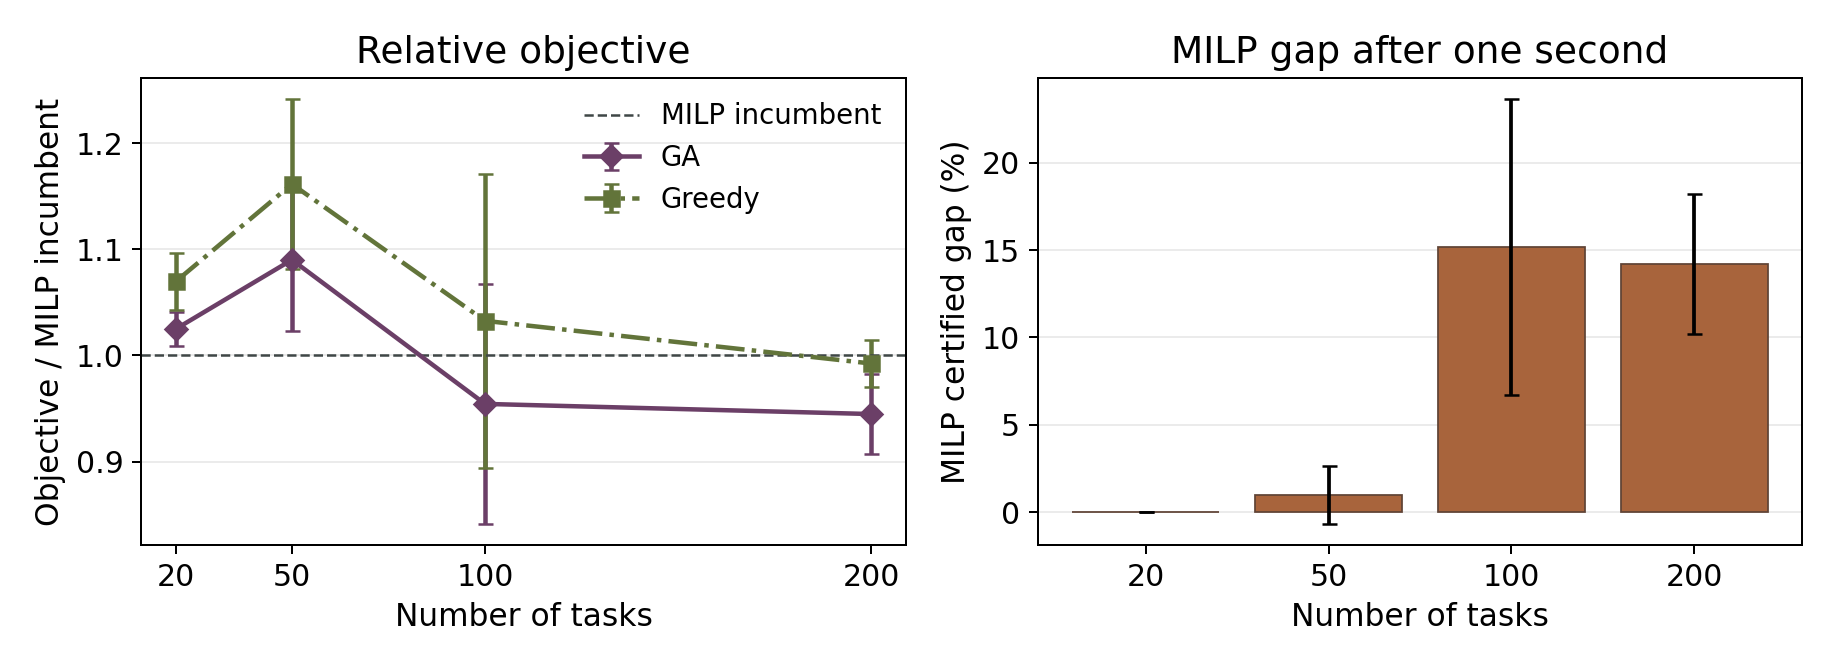
\includegraphics[width=\textwidth]{results/comparison.png}
\caption{Left: mean ratio to the MILP incumbent, paired by instance. Error bars
show the standard deviation across the three instance means. Right: the mean
MILP proof gap, with standard deviation across instances. A ratio below one
means a lower measured objective than the one second MILP incumbent.}
\label{fig:comparison}
\end{figure}

Greedy took under 0.003 seconds at every size; GA used about one second. MILP
took 0.10, 0.86 and slightly over one second for the 20, 50 and larger task
groups respectively, including model construction outside the solver limit.
These timings come from one computer. GA improved on greedy in mean objective
at every size. Its average within instance standard deviation was 5.5 CU
at 20 tasks and 28.5 CU at 200 tasks; the latter runs completed a median
of only three generations.
Those few generations make it difficult to attribute the result to extended
evolutionary search. Initial construction, repair and local moves are also part
of the method being measured.

The nominal allowances do not give identical end-to-end time budgets:
MILP model construction is outside its solver limit, while GA initialisation
is inside its search allowance. The measured wall times make this distinction
visible. These experiments compare solution quality under short search
allowances; they do not establish compliance with a strict one second deadline.

\Needspace{6\baselineskip}
Table~\ref{tab:resources} reports checked feasibility and mean peak resource
use. The balance column is $25z$.

\begin{table}[htbp]
\centering
\caption{Feasibility, resource use and wall time under the one second limit.}
\label{tab:resources}
\small
\begin{tabular}{rlrrrrrr}
\toprule
Tasks & Method & Feasible & Active & Peak CPU & Peak mem. & Balance & Time (s) \\
\midrule
20  & Greedy & 3/3   & 2.00  & 0.992 & 0.848 & 24.79 & 0.0002 \\
20  & GA     & 15/15 & 2.00  & 0.842 & 0.907 & 21.06 & 1.0010 \\
20  & MILP   & 3/3   & 2.00  & 0.874 & 0.948 & 21.86 & 0.0999 \\
50  & Greedy & 3/3   & 5.00  & 1.000 & 0.995 & 25.00 & 0.0007 \\
50  & GA     & 15/15 & 4.67  & 0.951 & 0.978 & 23.77 & 1.0021 \\
50  & MILP   & 3/3   & 4.33  & 0.992 & 1.000 & 24.79 & 0.8593 \\
100 & Greedy & 3/3   & 10.00 & 1.000 & 1.000 & 25.00 & 0.0008 \\
100 & GA     & 15/15 & 10.00 & 1.000 & 0.996 & 25.00 & 1.0036 \\
100 & MILP   & 3/3   & 10.67 & 1.000 & 0.983 & 25.00 & 1.0358 \\
200 & Greedy & 3/3   & 19.33 & 1.000 & 1.000 & 25.00 & 0.0029 \\
200 & GA     & 15/15 & 19.00 & 1.000 & 0.997 & 25.00 & 1.0104 \\
200 & MILP   & 3/3   & 21.33 & 1.000 & 0.991 & 25.00 & 1.1308 \\
\bottomrule
\end{tabular}
\end{table}

\subsection{Costs and resource use}

The 200 task results help explain the objective difference. MILP's one second
incumbents used a mean 21.3 servers, while the GA used 19.0 and greedy used
19.3. GA therefore paid a lower mean activation cost (1659.9) than the MILP
incumbent (1842.3), although its mean running cost was higher (1104.8 versus
1086.2). The net objective favoured GA at the time limit. Mean peak CPU and
memory utilisation were effectively one in all three methods at this size, so
the balance penalty was 25 in most allocations. These are averages across the
three instances, with five GA runs per instance.

\subsection{Sensitivity of the model}\label{sec:model-sensitivity}

I changed one parameter at a time on the 20 task, seed 11 instance and allowed
ten seconds for MILP to prove each result. The baseline optimum was 323.61 with
two active servers. Halving or doubling the activation costs changed the
objective to 234.61 or 501.61, but the chosen two server allocation did not
change. This shows that the baseline decision was stable over that particular
range; it does not imply activation costs are unimportant generally. Reducing
both capacity types by 10\% raised the optimum to 327.04, while increasing them
by 10\% lowered it to 321.45. Reducing all task CPU and memory demands by
10\% lowered the optimum to 321.26; increasing them by 10\% raised it to
326.81. Assignment costs were held fixed in these demand tests to isolate the
effect of resource limits. Setting $\lambda=0$ allowed a peak CPU
utilisation of 1.00; setting it to 50 reduced the peak to 0.825. The
corresponding objective values cannot be compared as pure placement costs
because the objective function itself changes with $\lambda$.

\begin{table}[htbp]
\centering
\caption{Changes to the model on the 20 task, seed 11 instance. Every result was proved optimal with a ten second solver allowance.}
\label{tab:model-sensitivity}
\small
\begin{tabular}{lrrrr}
\toprule
Change from baseline & Objective (CU) & Active & Peak CPU & Peak memory \\
\midrule
None & 323.61 & 2 & 0.844 & 0.985 \\
Activation charges $\times0.5$ & 234.61 & 2 & 0.844 & 0.985 \\
Activation charges $\times2$ & 501.61 & 2 & 0.844 & 0.985 \\
Both capacities $\times0.9$ & 327.04 & 2 & 0.938 & 0.995 \\
Both capacities $\times1.1$ & 321.45 & 2 & 0.750 & 0.950 \\
Both demands $\times0.9$ & 321.26 & 2 & 0.743 & 0.940 \\
Both demands $\times1.1$ & 326.81 & 2 & 0.928 & 0.985 \\
$\lambda=0$ CU & 300.51 & 2 & 1.000 & 0.925 \\
$\lambda=50$ CU & 344.46 & 2 & 0.825 & 0.970 \\
\bottomrule
\end{tabular}
\end{table}

The last two rows show the intended meaning of the peak penalty. Increasing
$\lambda$ reduces the chosen CPU peak, but the direct activation and assignment
cost also matters. That direct cost is 300.51 CU when $\lambda=0$, 302.52 CU
at the baseline weight, and 303.21 CU when $\lambda=50$. The larger weight
therefore buys more CPU headroom at a slightly larger placement charge. It does
not enforce a particular peak or guarantee a similar change on every instance.
The capacity and demand changes also affect normalised CPU utilisation, so their
objective changes include both feasibility and peak cost effects.

\subsection{Experimental design for GA settings}

The model sensitivity study changes the allocation problem. The following
study instead holds the problem fixed and changes how the GA searches it.
This distinction matters because a lower cost under a different objective is
not evidence of a better algorithm. Fixed parameter tuning and parameters that
change during a run are also different approaches \cite{eiben1999}. Here each
setting stays fixed throughout a run.

I use the 100 task, 12 server and 200 task, 24 server instances, with instance
seeds 11, 22 and 33. Each configuration receives five GA runs on each of those
six instances. All runs use three seconds, including initialisation, so a larger
population must justify its cost within the same allowance. The study has
$11\times6\times5=330$ runs. Settings are changed one at a time from
Table~\ref{tab:ga-settings}: population size 12 or 48; tournament size 2 or 5;
rank selection; crossover probability 0 or 0.6; and mutation probability 0,
0.01 or 0.08. The baseline is included. Decoder retention, score noise, ordering
jitter, two elites and the local improvement pass stay at their defaults.

Within an instance and repetition, configurations use the same initial random
seed, $1000s+r+16$, where $s$ is the instance seed and $r=1,\ldots,5$.
The execution order is shuffled using order seed 20260929, with every run
executed sequentially. This avoids making a particular configuration always
run first or last. Common seeds give comparable starting conditions, although
different operators consume random draws differently and do not follow
identical search paths. Exact runtime limited results can also change slightly
when the machine load changes.

For configuration $\theta$, task count $n$, instance seed $s$ and repetition
$r$, I calculate
\[
d_{n,s,r}(\theta)=100\left(\frac{C_{n,s,r}(\theta)}{C_{n,s,r}(\mathrm{baseline})}-1\right).
\]
A negative value means a cheaper result under the same objective and time
allowance. The tables report mean cost, mean paired percentage change and
the average within instance sample standard deviation of the five costs.
The last measure describes randomness in the GA, rather than differences
between workloads. I also save initialisation time, completed generations,
accepted and rejected offspring, and a trace of each best cost improvement.
Every saved allocation is checked again from its instance JSON.

The configuration with the smallest mean $d_{n,s,r}$ across the two sizes is
selected using only these tuning cases, giving equal weight to each size and
instance. It is then compared with the baseline on new instance seeds
44, 55 and 66, again at both sizes with five runs and three seconds per run.
That validation adds 60 runs. It tests transfer to six unseen workloads from
the same generator, rather than selecting a configuration using its validation
results. One parameter at a time makes the comparison interpretable but does
not search interactions between parameters, a limitation discussed in the
parameter setting literature \cite{eiben1999}.

\subsection{Results of the GA setting study}

Table~\ref{tab:ga-tuning} shows that the settings change both mean cost and
run variation. All 330 runs returned feasible allocations. Every initial
population reached its target size, and none of the 101877 attempted offspring
repairs failed on these samples. These checks concern the generated workloads;
they do not establish a general feasibility guarantee for the decoder.
In the tuning runs, mean wall times were about 3.00 seconds at 100 tasks and 3.01 seconds at 200,
with a largest observed overrun of 0.093 seconds while an operation finished.

\begin{table}[htbp]
\centering
\small
\caption{GA settings at three seconds. Each size has three instances and five runs per setting. Cost and SD are in CU; SD is the average within instance sample standard deviation. Change is the mean paired percentage change from the default.}
\label{tab:ga-tuning}
\begin{tabular}{lrrrrrr}
\toprule
& \multicolumn{3}{c}{100 tasks, 12 servers} & \multicolumn{3}{c}{200 tasks, 24 servers} \\
\cmidrule(lr){2-4}\cmidrule(lr){5-7}
Setting & Cost & Change (\%) & SD & Cost & Change (\%) & SD \\
\midrule
Default & 1457.36 & $0.00$ & 14.63 & 2744.66 & $0.00$ & 14.13 \\
Population $N_{\rm pop}=12$ & 1444.89 & $-0.81$ & 29.31 & 2744.68 & $0.00$ & 30.49 \\
Population $N_{\rm pop}=48$ & 1457.63 & $+0.02$ & 14.15 & 2758.87 & $+0.53$ & 27.37 \\
Tournament $k=2$ & 1449.44 & $-0.51$ & 14.03 & 2751.49 & $+0.26$ & 12.89 \\
Tournament $k=5$ & 1446.25 & $-0.74$ & 25.74 & 2726.22 & $-0.67$ & 18.38 \\
Rank selection & 1447.78 & $-0.62$ & 27.87 & 2755.95 & $+0.41$ & 33.11 \\
Crossover $p_c=0$ & 1438.02 & $-1.27$ & 25.10 & 2731.35 & $-0.48$ & 22.12 \\
Crossover $p_c=0.6$ & 1442.30 & $-1.00$ & 23.91 & 2737.08 & $-0.29$ & 27.37 \\
Mutation $p_m=0$ & 1435.86 & $-1.44$ & 29.14 & 2732.71 & $-0.44$ & 18.96 \\
Mutation $p_m=0.01$ & 1435.62 & $-1.46$ & 29.94 & 2729.42 & $-0.55$ & 28.23 \\
Mutation $p_m=0.08$ & 1464.69 & $+0.52$ & 0.93 & 2775.86 & $+1.18$ & 23.15 \\
\bottomrule
\end{tabular}
\end{table}


\paragraph{Population and selection.}
Doubling the population from 24 to 48 did not improve mean cost at either size.
At 200 tasks its mean cost was 0.53\% higher than the paired default.
The smaller population of 12 improved the 100 task mean by 0.81\%, but made
almost no difference at 200 tasks and increased run variation. At 100 tasks,
populations 12, 24 and 48 completed means of 48.5, 20.4 and 9.8 full
generations; at 200 tasks the figures were 14.5, 6.3 and 2.8. A generation
contains a different number of children at each population size. The mean
accepted offspring counts were much closer: about 489, 458 and 473 at
100 tasks, and 150, 149 and 147 at 200. More generations therefore did not
mean a proportional increase in candidate allocations. Larger populations
also spent more of the allowance in initialisation.

Tournament size 5 lowered the paired mean by 0.74\% at 100 tasks and 0.67\%
at 200. Tournament size 2 and rank selection had lower means at 100 tasks
but slightly higher means at 200. Stronger selection was useful on these
tuning cases, although these differences are too limited to establish a
generally preferred selection rule.

\paragraph{Crossover and mutation.}
Skipping crossover improved the tuning means by 1.27\% and 0.48\%; using
crossover probability 0.6 improved them by 1.00\% and 0.29\%. These results
show that uniform crossover was not automatically helpful under this short
allowance and repair rule. They do not show that genetic recombination is
ineffective generally. The decoder still changes preferences and the local
pass still improves repaired children, even when crossover is skipped.

Mutation rate 0.01 had the lowest mean paired change when both sizes were
weighted equally: a 1.00\% reduction. Its mean costs were 1435.62 and
2729.42 CU, compared with the default's 1457.36 and 2744.66 CU.
The average within instance SD increased from 14.63 to 29.94 CU at
100 tasks and from 14.13 to 28.23 CU at 200. Thus a lower average cost
came with more variability. Mutation rate 0 was close behind on the tuning
criterion. The high rate 0.08 raised mean cost at both sizes. Its small
100 task SD of 0.93 CU describes consistency, but that consistency came
with a more expensive mean allocation.

Figure~\ref{fig:ga-settings} retains the differences between workloads.
For mutation rate 0.01, the paired improvements at 100 tasks were 0.16\%,
1.25\% and 2.97\% on seeds 11, 22 and 33. The latter two cases saved mean
activation charges of 20.2 and 48.0 CU, while paying slightly more in
assignment charges. Occasional better consolidation therefore accounts for
much of the mean improvement. The effect is not uniform across instances.

One possible explanation is that independent crossover and resets disrupt
groups of tasks sharing a cheap server. A feasible repair need not restore
those groups, and a single task move cannot always empty a server whose
tasks would have to move together. This interpretation agrees with the
observed cost components: at 200 tasks, mutation rate 0.08 paid a mean
31.2 CU more in activation charges than the default, while their mean
assignment charges were almost identical. The experiment does not isolate
each mechanism, so it supports this explanation without proving it.

\begin{figure}[htbp]
\centering
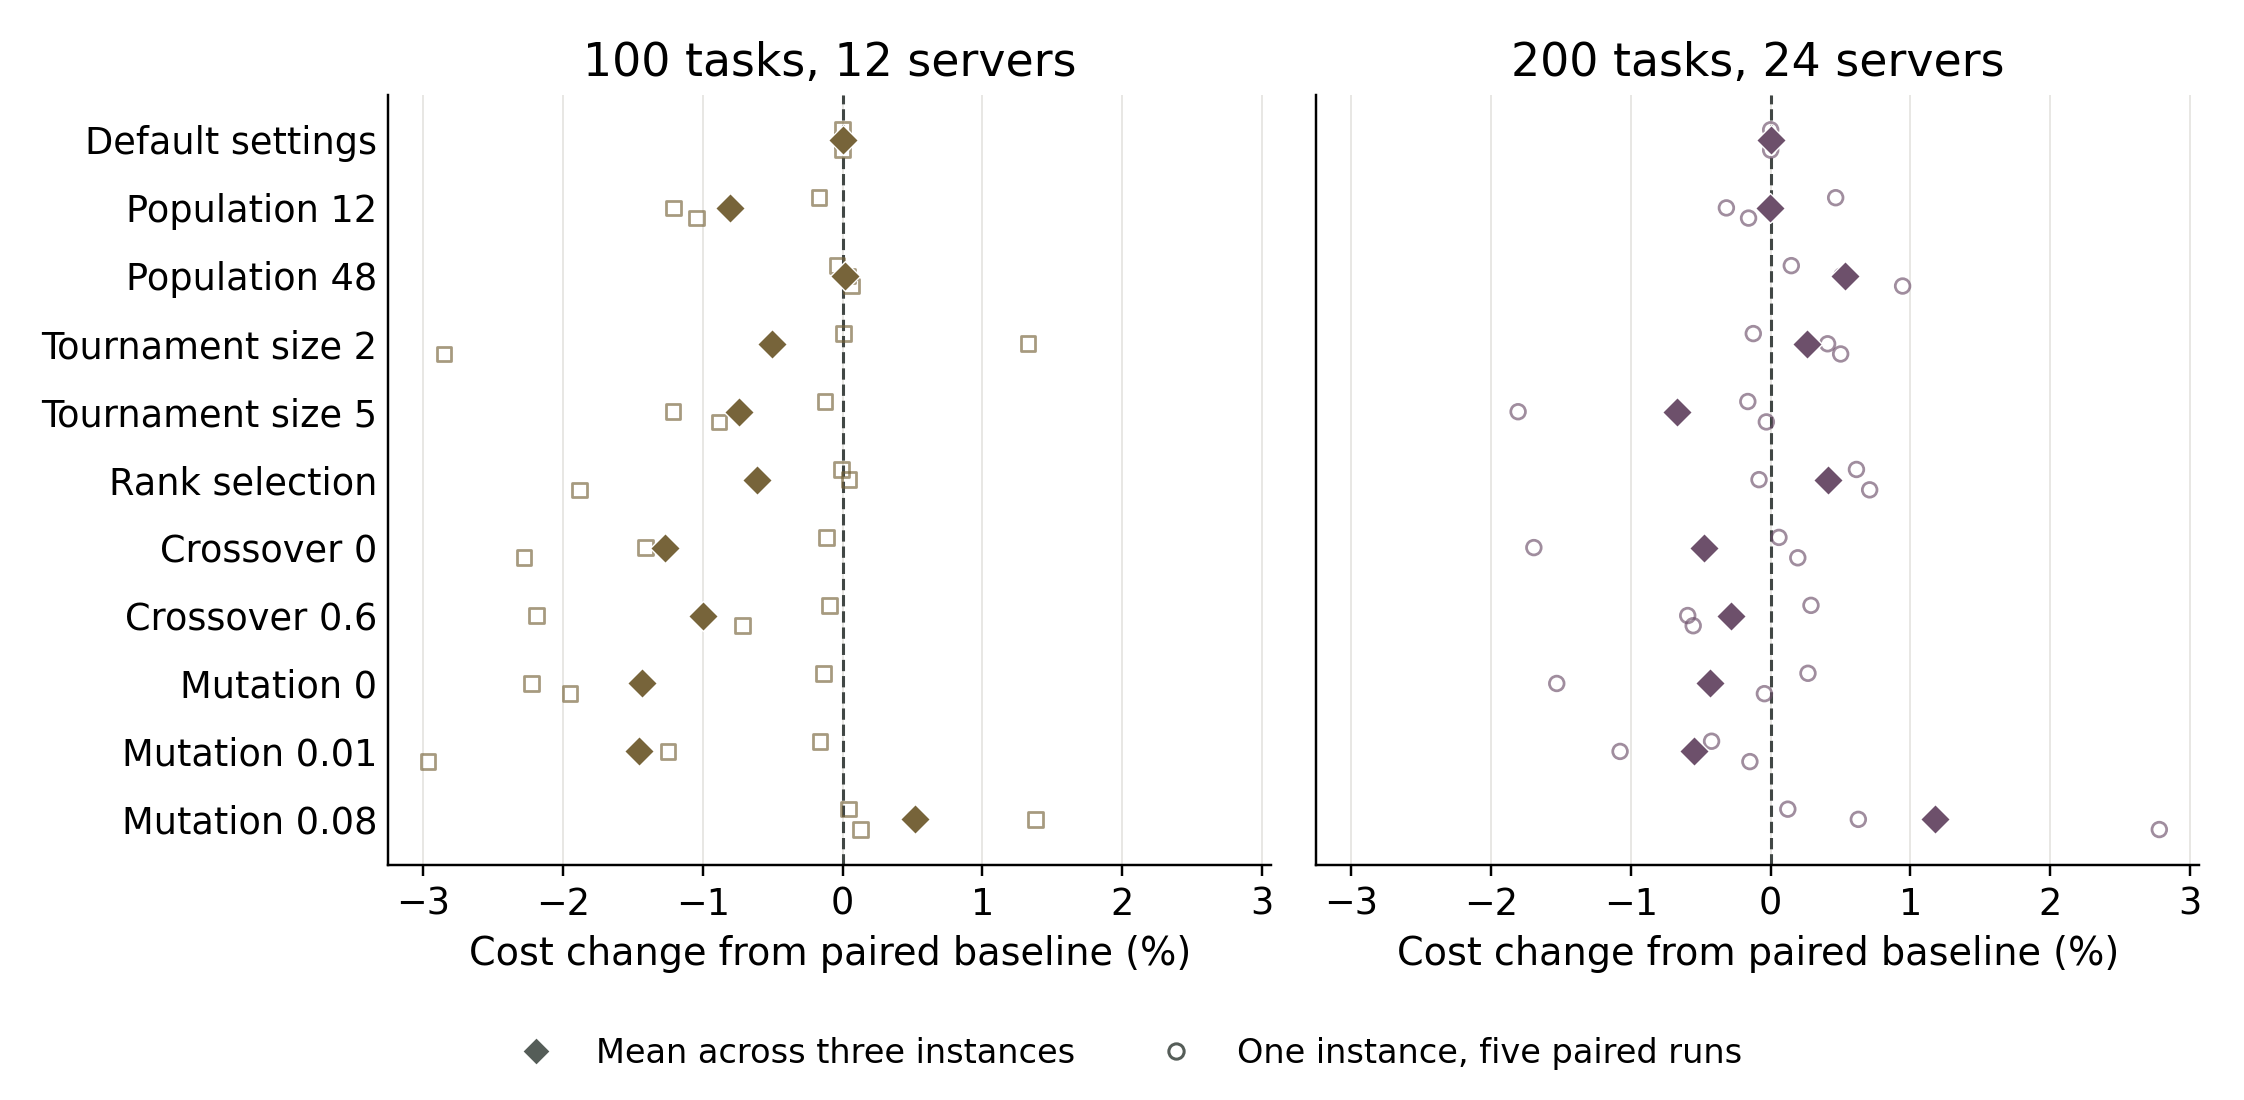
\includegraphics[width=\textwidth]{ga_tuning/parameter_changes.png}
\caption{Paired changes in GA cost at three seconds. Each hollow marker is an
instance's mean across five paired runs; each solid diamond averages the three
instance means. Negative values favour the changed setting. These markers
describe instance variation, not confidence intervals.}
\label{fig:ga-settings}
\end{figure}

\paragraph{Validation on new instances.}
The selected setting changes only $p_m$ to 0.01. Table~\ref{tab:ga-validation}
uses seeds 44, 55 and 66, which were excluded from selection. All 60
validation runs were feasible. The pooled paired change was $+0.006\%$,
effectively zero: $+0.020\%$ at 100 tasks and $-0.007\%$ at 200 tasks.
The selected setting had a lower mean cost on three of the six workloads
and won 17 of the 30 paired runs. These repeated runs share only six
workloads, so they are not 30 independent tests of transfer to different data.

\begin{table}[htbp]
\centering
\small
\caption{Validation on unseen instance seeds at three seconds, with five runs per cell. SD is the sample standard deviation within that instance, in CU. Changes pair identical instance and run seeds.}
\label{tab:ga-validation}
\begin{tabular}{rrrrrrr}
\toprule
Tasks & Seed & Default (CU) & Selected (CU) & Change (\%) & Default SD & Selected SD \\
\midrule
100 & 44 & 1582.65 & 1583.13 & $+0.03$ & 1.64 & 1.42 \\
100 & 55 & 1320.61 & 1318.80 & $-0.14$ & 2.31 & 3.72 \\
100 & 66 & 1532.72 & 1535.25 & $+0.17$ & 2.47 & 1.97 \\
200 & 44 & 2800.63 & 2800.11 & $-0.02$ & 4.42 & 1.15 \\
200 & 55 & 2787.57 & 2793.37 & $+0.21$ & 18.19 & 19.57 \\
200 & 66 & 2881.72 & 2875.44 & $-0.22$ & 3.53 & 11.14 \\
\bottomrule
\end{tabular}
\end{table}


The tuning gain did not transfer consistently to the new seeds. I therefore
retain the original default rate for the main comparison and treat 0.01 as
a candidate for a particular workload, rather than a generally improved
setting. The validation set was not used to choose a second winner.
This outcome is useful: settings that look favourable on a small tuning set
can make almost no difference on another set from the same generator.
The study is limited to three seconds, two sizes and one parameter at a time;
it does not identify an optimum over all GA settings or their interactions.

\Needspace{7\baselineskip}
The validation can be repeated with the study script using
\begin{verbatim}
python3 run_ga_study.py --phase validation \
  --configs baseline mutation_001 --budget 3 \
  --repetitions 5 --output ga_validation_new
\end{verbatim}
The raw records, saved assignments and improvement traces support these
comparisons, including the validation result that did not favour the tuning
winner overall.


\subsection{Using the MILP bound with a GA result}

Let $D$ be the solver's dual bound and $U$ the cost of a feasible GA allocation.
Then $D\leq v^\star\leq U$, and
\[
0\leq\frac{U-v^\star}{U}\leq\frac{U-D}{U}.
\]
I use a gap normalised by the feasible cost $U$, as in the reported MILP gaps.
If error were instead measured relative to the unknown optimum, the valid
upper bound would be $(U-D)/D$ for $D>0$. These ratios are unitless because
their numerators and denominators are costs in the same units.
SciPy exposes $D$ as \texttt{mip\_dual\_bound} and reports the solver's own
gap relative to its primal objective \cite{scipymilp}. Here I substitute the
checked GA cost as the feasible upper bound. I paired the bound after
the experiments with the first GA run on each
instance. For the 100 task group, the mean remaining gap between that GA cost
and the MILP lower bound was 10.9\%, compared with a mean 15.2\% certified gap
for the MILP's own assignment. For 200 tasks, the figures were 9.2\% and
14.2\%. The calculation uses $(\text{GA cost}-\text{MILP bound})/
\text{GA cost}$ on each instance before averaging. It shows how a good heuristic
answer and a mathematical bound can complement each other. These are separate
one second runs, so this is roughly two seconds of post hoc analysis, not a
tested one second hybrid scheduler.

\subsection{Running the code with different data}

The model and algorithms are in \texttt{scheduler.py}, with separate scripts
for experiments, plots and checks. The project requires Python 3.11 or later.
From the project folder, a small run can be made with
\begin{verbatim}
python3 -m pip install -r requirements.txt
python3 run_experiments.py --sizes 20x4 --seeds 11 \
  --budget 1 --repetitions 1 --output local_results
\end{verbatim}
The benchmark writes raw CSV, instances, allocations and version details to
the chosen output directory. The saved full benchmarks are in \texttt{results/}
and \texttt{results\_3s/}; the setting studies are in \texttt{ga\_tuning/}
and \texttt{ga\_validation/}.
New instance sizes and seeds can be passed with, for example,
\texttt{-{}-sizes 30x5 80x10 -{}-seeds 4 5}. Use a new output directory
to keep a run separate from the saved results. Individual GA settings can be
changed with \texttt{-{}-population}, \texttt{-{}-selection},
\texttt{-{}-tournament}, \texttt{-{}-crossover} and \texttt{-{}-mutation}.
Running \texttt{run\_experiments.py} or \texttt{run\_ga\_study.py} with
\texttt{-{}-help} lists the options.

\Needspace{11\baselineskip}
The saved allocations and bounds can be checked without rerunning the time
limited searches:
\begin{verbatim}
python3 verify_results.py --results results
python3 verify_results.py --results results_3s
python3 run_ga_study.py --verify ga_tuning
python3 run_ga_study.py --verify ga_validation
\end{verbatim}
The repository includes the measured inputs, allocations, raw tables, settings
and improvement traces. Repeating a timed run uses the same data and random seed
rules, but it need not reproduce exactly the same incumbent because the number
of operations completed depends on machine load.

For external data, use a JSON file with consistent units. A three task example is
\begin{verbatim}
{
  "task_cpu": [4, 3, 2], "task_mem": [8, 6, 4],
  "server_cpu": [7, 8], "server_mem": [12, 15],
  "fixed_cost": [25, 30],
  "assignment_cost": [[3, 5], [4, 3], [2, 4]],
  "balance_weight": 12
}
\end{verbatim}
Run \texttt{python3 run\_experiments.py -{}-instance my\_instance.json} with
the desired budget, repetitions and output directory. The assignment cost
array has one row per task and one column per server. Demands, capacities and
charges must be positive and finite; the balance weight may be zero. Assignment
JSON files contain one zero based server index per task, in input order.
A blank objective means that the method did not return a checked feasible
allocation. For MILP, the status, bound and gap distinguish an incumbent from
an allocation whose optimality was proved.

\section{Final discussion}

The main result depends on the time allowed. For the smallest instances, the MILP
provides both a good allocation and proof that no better one exists. Under a
one second limit on the largest instances, it still supplies a feasible answer
and a lower bound, but its certified 14 to 15\% gap leaves room for improvement.
The GA used that time to find cheaper feasible placements on average, while
greedy supplied an answer almost immediately. At three seconds, MILP had the
lower mean cost for 100 tasks, while GA retained the advantage at 200. Neither
large group was proved optimal. This suggests a practical sequence for this
specific model: keep a greedy allocation as a fallback, run MILP when proof is
valuable and time is available, and consider GA when the deadline is short and
the instance is large.

There are important limits to that conclusion. I used synthetic data, three
instances per size and one computer. The crossover point may move with task
sizes, cost ranges, server heterogeneity, or a longer time limit. The GA includes
local improvement, so the measured gain is not due to crossover alone. The
current peak CPU penalty becomes constant when a server fills, and memory is
not explicitly balanced. A future model could include time windows, migration
costs, uncertain task demand or a more informative load measure. A useful next
experiment would give a single total time budget to a short MILP run followed
by GA search seeded with its incumbent. The same budget should also be given
to MILP and GA individually.

The GA setting study adds a different conclusion. Lower mutation and less
crossover sometimes reduced cost on the tuning cases, often through better
consolidation, but the selected mutation rate gave effectively no overall
improvement on the six new workloads. Increasing population size also did not
automatically help under three seconds. The comparison needs both final cost
and its variation, together with the amount of search completed. I retain the
original defaults rather than changing them on the strength of the tuning mean.
More instances, different demand profiles and longer allowances would be needed
before recommending a setting beyond this experiment. The one second method
comparison and the three second parameter study answer related but distinct
questions.

The accompanying code, saved instances and allocations make every number in
this report traceable to a run.

\clearpage
\begin{thebibliography}{9}
\small
\bibitem{beloglazov2012}
A. Beloglazov, J. Abawajy, and R. Buyya, ``Energy-aware resource allocation
heuristics for efficient management of data centers for Cloud computing,''
\emph{Future Generation Computer Systems}, vol. 28, no. 5, pp. 755--768, 2012.
\url{https://doi.org/10.1016/j.future.2011.04.017}.

\bibitem{johnson1974}
D. S. Johnson, ``Fast algorithms for bin packing,''
\emph{Journal of Computer and System Sciences}, vol. 8, no. 3, pp. 272--314,
1974. \url{https://doi.org/10.1016/S0022-0000(74)80026-7}.

\bibitem{scipymilp}
SciPy Developers, ``\texttt{scipy.optimize.milp} reference,''
\url{https://docs.scipy.org/doc/scipy-1.16.2/reference/generated/scipy.optimize.milp.html},
accessed 3 October 2026.

\bibitem{highs}
HiGHS project, ``HiGHS: High performance software for linear optimization,''
\url{https://highs.dev/}, accessed 25 September 2026.

\bibitem{holland1992}
J. H. Holland, \emph{Adaptation in Natural and Artificial Systems}.
MIT Press, 1992.
\url{https://mitpress.mit.edu/9780262581110/adaptation-in-natural-and-artificial-systems/}.

\bibitem{whitley1994}
D. Whitley, ``A genetic algorithm tutorial,'' \emph{Statistics and Computing},
vol. 4, no. 2, pp. 65--85, 1994.
\url{https://doi.org/10.1007/BF00175354}.

\bibitem{eiben1999}
A. E. Eiben, R. Hinterding, and Z. Michalewicz,
``Parameter control in evolutionary algorithms,''
\emph{IEEE Transactions on Evolutionary Computation},
vol. 3, no. 2, pp. 124--141, 1999.
\url{https://doi.org/10.1109/4235.771166}.

\end{thebibliography}

\end{document}
